\chapter{Ausarbeitung}
\section{Aufgabe 1}
Die Drehraten sind von der Erdrotation befreit: $\omega_e = 0$, das gilt:
\begin{equation*}
	\bm{\omega}_{ep}^p = \bm{\omega}_{ip}^p
\end{equation*}
$\bm{\omega}_{ip}^p$ sind die gemessene Drehraten, die Elementen von $\bm{A}$ Matrix sind bekannt. 
\begin{gather*}
	\bm{q}(t+\Delta t) = e^{\frac{\bm{A} \Delta t}{2}} \cdot \bm{q}(t) \\
	\bm{q}(0) = \begin{bmatrix}
		1 \\
		0 \\
		0 \\
		0
	\end{bmatrix}
\end{gather*}
Für jede Epoche sind dann DCM mit $\bm{q}$ bestimmbar, dann gibt es:
\begin{gather*}
	\bm{g}^{e} = -9,81 \cdot \frac{\bm{x}}{|\bm{x}|} \\
	\dot{\bm{v}}^{e} = \bm{C} \bm{a}^{p} + \bm{g}^{e} \\
	\bm{v}^{e}(t) = \bm{v}^{e}(t-1) + \dot{\bm{v}}^{e} \cdot \Delta t \\
	\bm{x}^{e}(t) = \bm{x}^{e}(t-1) + \bm{v}^{e} \cdot \Delta t
\end{gather*}
Die Trajektorie liegt in \autoref{fig:Trajektorie}. Sie liegt in x-z Ebene und wölbt sich nach innen. 
\begin{figure}[htbp]
	\centering
	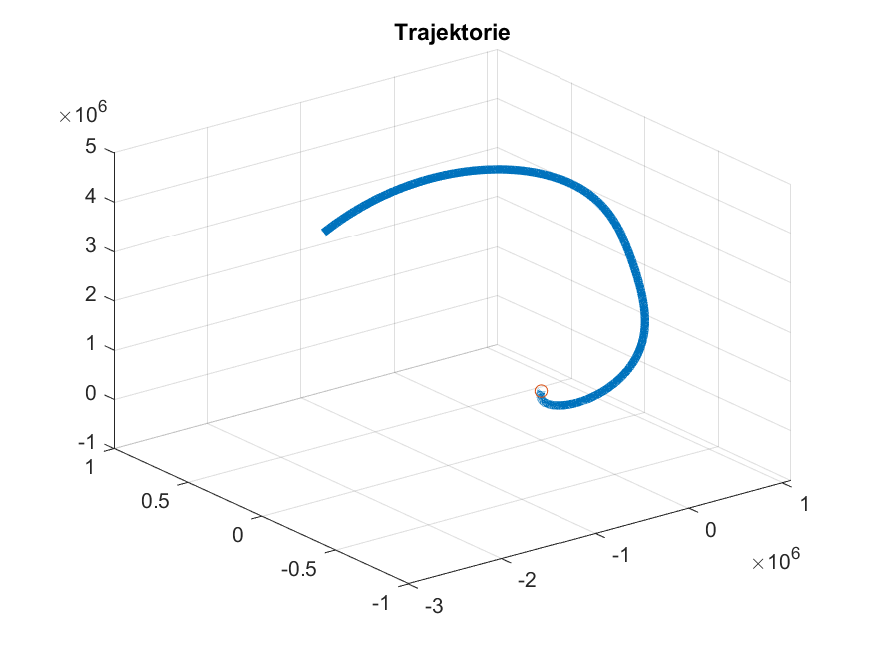
\includegraphics[width=0.9\textwidth]{images/Trajektorie} 
	\caption{Trajektorie} 
	\label{fig:Trajektorie}
\end{figure}\\\\
$\sqrt{x^2 + y^2 + z^2}$ sind immer kleiner als Erdradius, deswegen ist der Verlauf nicht realistisch.
\clearpage
\section{Aufgabe 2}
Analog wie Aufgabe 1, die Positionen werden rückwärts geschätzt. 
\begin{gather*}
	\bm{\omega}_{rueck} = - \bm{\omega}_{vor} \\
	\bm{a}_{rueck} = - \bm{a}_{vor} \\
	\bm{v}_{rueck}(1) = \bm{v}_{vor}(end)
\end{gather*} 
Die Biasoffset hat 8 Möglichkeiten:
\begin{align*}
	\delta a_1 & = [0,1\quad 0,1\quad 0,1] \\
	\delta a_2 & = [0,1\quad 0,1\quad -0,1] \\
	\delta a_3 & = [0,1\quad -0,1\quad 0,1] \\
	\delta a_4 & = [0,1\quad -0,1\quad -0,1] \\
	\delta a_5 & = [-0,1\quad 0,1\quad 0,1] \\
	\delta a_6 & = [-0,1\quad 0,1\quad -0,1] \\
	\delta a_7 & = [-0,1\quad -0,1\quad 0,1] \\
	\delta a_8 & = [-0,1\quad -0,1\quad -0,1] \\
\end{align*}
Die Ursprünliche Position werden berechnet
\begin{table}[htpb] \centering
	\begin{tabular}{llll}
		bias offset & $x_1$    & $x_2$   & $x_3$   \\
		$\delta a_1$ & -4,60e04 & 4,25e3  & -1,29e5 \\
		$\delta a_2$ & -3,95e04 & -6,42e3 & -1,14e5 \\
		$\delta a_3$ & -4,60e04 & -4,25e3 & -1,29e5 \\
		$\delta a_4$ & -3,95e4  & 6,42e3  & -1,14e5 \\
		$\delta a_5$ & -1,33e5  & -9,38e3 & -2,45e5 \\
		$\delta a_6$ & -1,84e4  & 1,89e4  & -6,47e4 \\
		$\delta a_7$ & -1,33e5  & 9,38e3  & -2,45e5 \\
		$\delta a_8$ & -1,84e4  & -1,89e4 & -6,47e4
	\end{tabular}
\end{table}\\
Alle neu Trajektorie liegen in \autoref{fig:Trajektorie rückwärt}
\begin{figure}[ht]\centering
	\subfigure[$\delta a_1$]{
		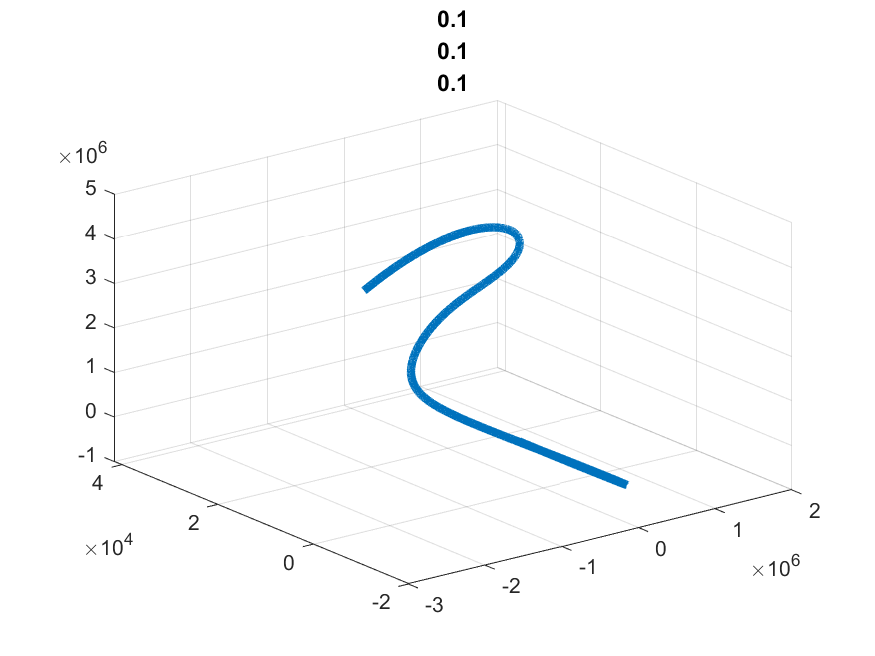
\includegraphics[width=0.45\textwidth]{1.png}}
	\subfigure[$\delta a_2$]{
		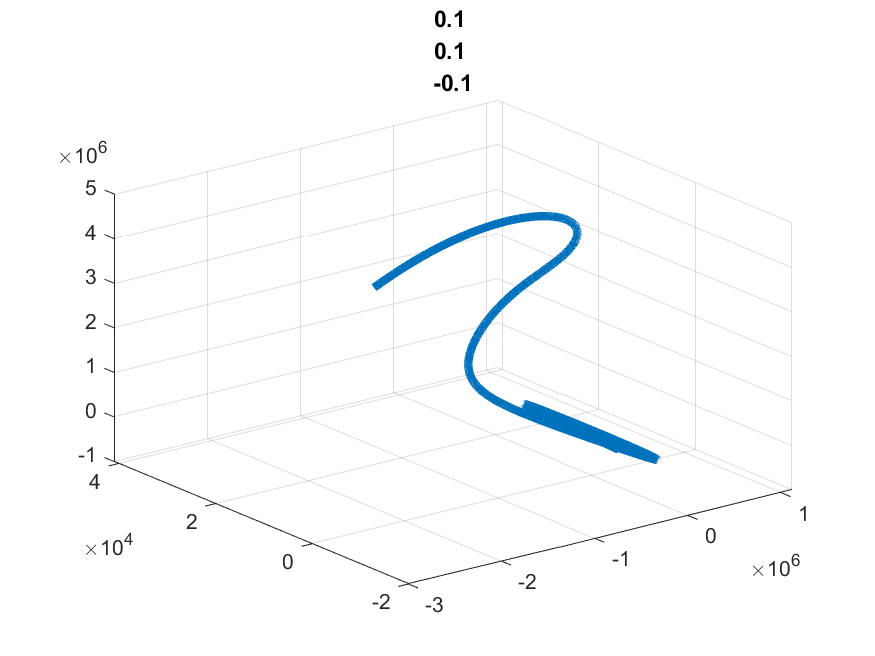
\includegraphics[width=0.45\textwidth]{2.png}}
	\subfigure[$\delta a_3$]{
		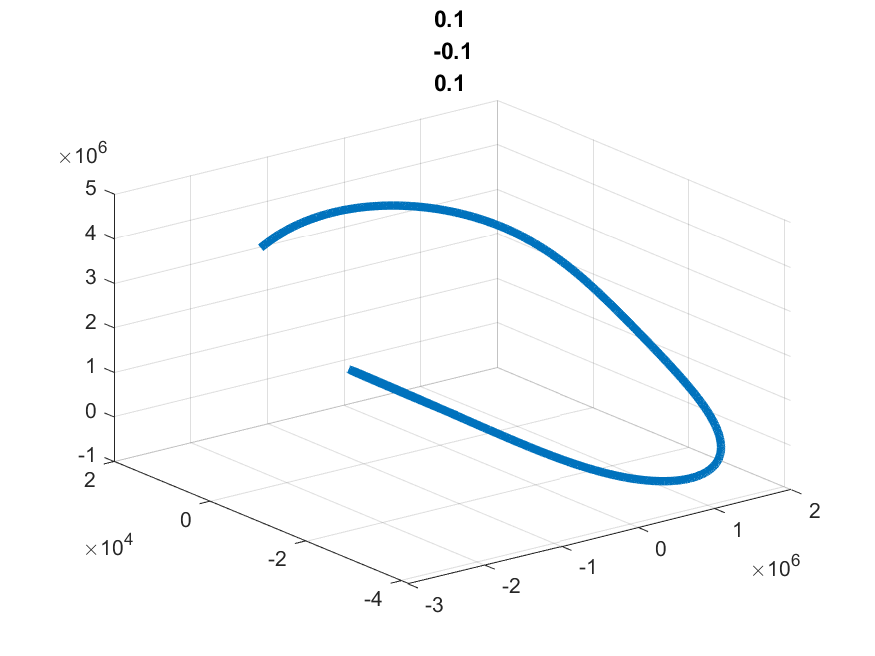
\includegraphics[width=0.45\textwidth]{3.png}}
	\subfigure[$\delta a_4$]{
		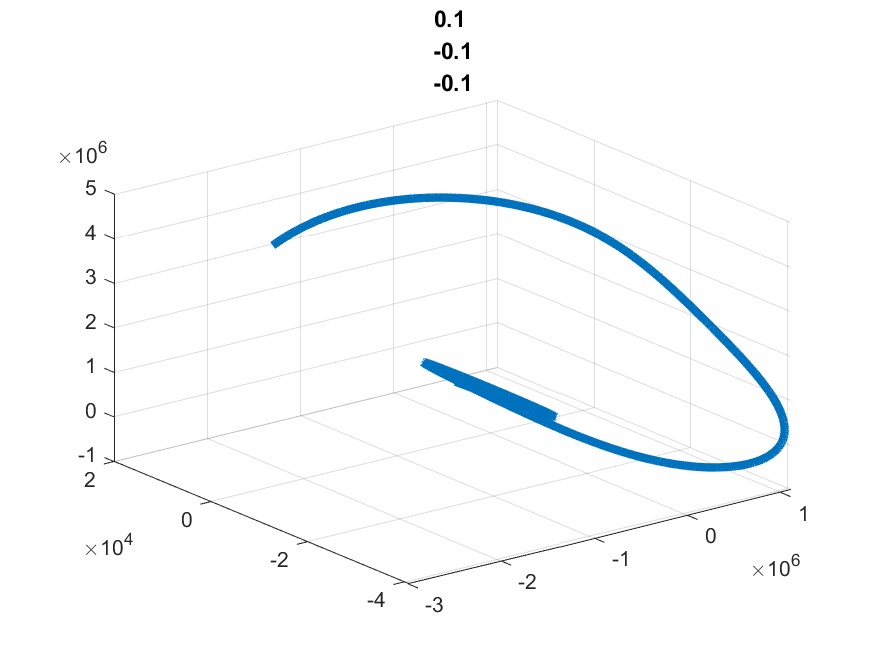
\includegraphics[width=0.45\textwidth]{4.png}}
	\subfigure[$\delta a_5$]{
		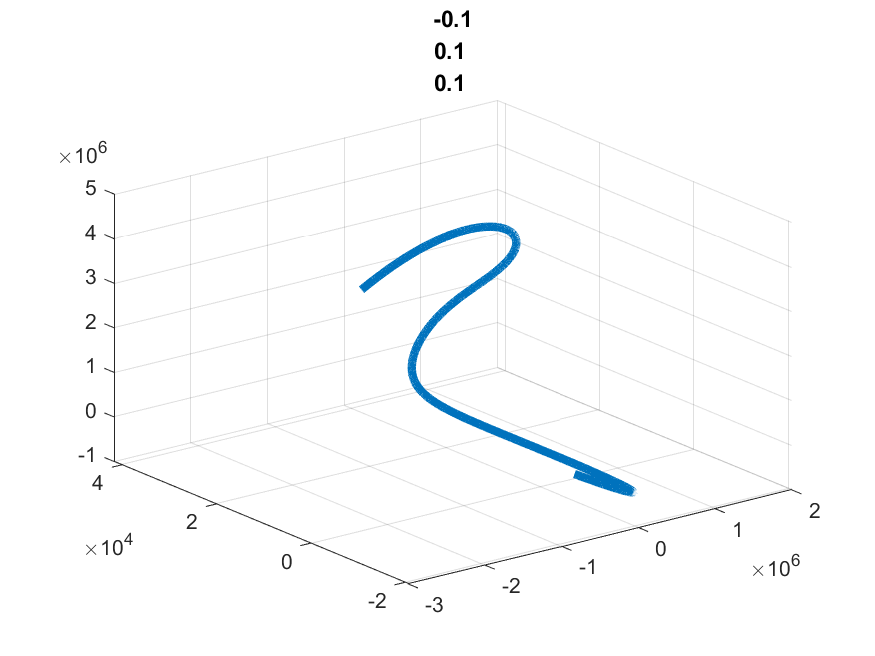
\includegraphics[width=0.45\textwidth]{5.png}}
	\subfigure[$\delta a_6$]{
		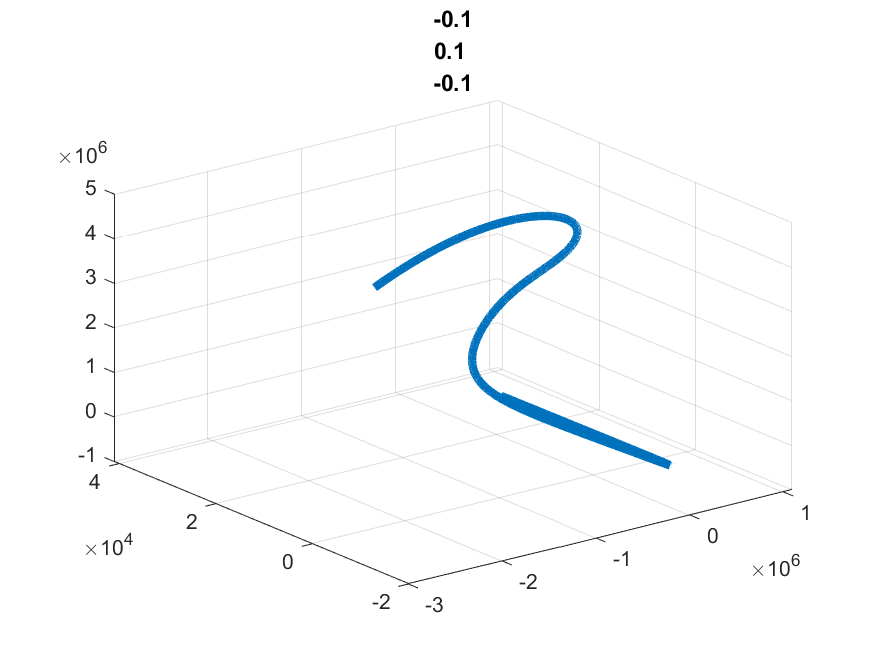
\includegraphics[width=0.45\textwidth]{6.png}}
	\subfigure[$\delta a_7$]{
		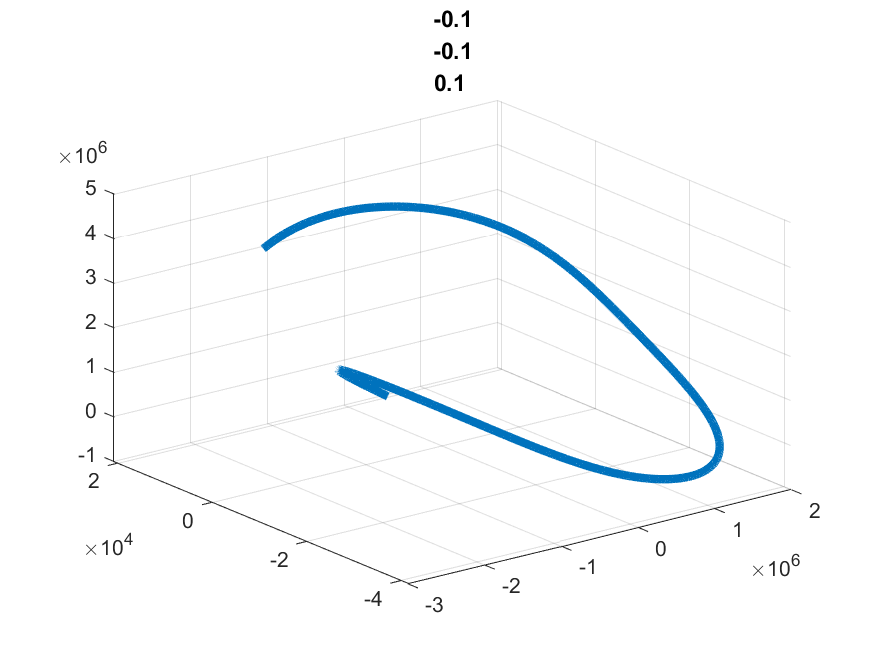
\includegraphics[width=0.45\textwidth]{7.png}}
	\subfigure[$\delta a_8$]{
		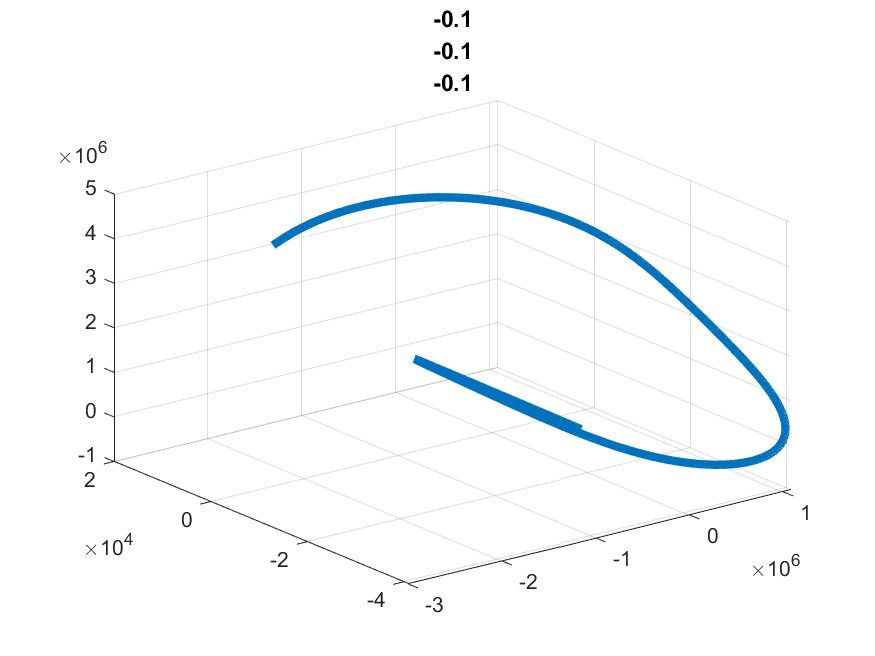
\includegraphics[width=0.45\textwidth]{8.png}}
	\label{fig:Trajektorie rückwärt}
\end{figure}
\clearpage
Die Streuung der Positionen:
\begin{table}[htpb] \centering
	\begin{tabular}{ll}
		Bias offset & Streuung [m] \\
		$\delta a_1$ & 1,37e5 \\
		$\delta a_2$ & 1,21e5 \\
		$\delta a_3$ & 1,37e5  \\
		$\delta a_4$ & 1,21e5  \\
		$\delta a_5$ & 2,79e5  \\
		$\delta a_6$ & 6,99e4  \\
		$\delta a_7$ & 2,79e5   \\
		$\delta a_8$ & 6,99e4 
	\end{tabular}
\end{table}\\
Es ist zu sehen, wenn die Bias Offset in x und y gleich sind, sind die Streuung auch gleich. Der Grund dafür ist: Sensor messt Beschleunigung nur in x und z Richtungen und Drehraten um y Achse. Deswegen hängen die y Koordinaten und die Geschwindigkeit in y Richtung nur von Bias offset und Gravitation ab. 










